\let\lesson\undefined
\newcommand{\lesson}{\phantomlesson{Bài 17: Động năng và thế năng. Định luật bảo toàn cơ năng}}
\chapter[Động năng và thế năng]{Động năng và thế năng}
\setcounter{section}{0}
\section{Lý thuyết}
\subsection{Động năng}
\subsubsection{Khái niệm động năng}
Động năng của một vật là năng lượng mà vật có được do nó đang chuyển động. 

Nếu vật khối lượng $m$ đang chuyển động với vận tốc $v$ thì động năng của vật được xác định theo công thức:
\begin{equation*}
	W_{\text{đ}} =\dfrac{1}{2}mv^2
\end{equation*}
trong đó:
\begin{itemize}
	\item $W_{\text{đ}}$: động năng, đơn vị trong hệ SI là joule $\left(\si{\joule}\right)$;
	\item $m$: khối lượng của vật, đơn vị trong hệ SI là kilogram $\left(\si{\kilogram}\right)$;
	\item $v$: tốc độ của vật, đơn vị trong hệ SI là $\si{\meter/\second}$.
\end{itemize}
\subsubsection{Đặc điểm của động năng}
\begin{itemize}
	\item Động năng là đại lượng vô hướng, không âm.
	\item Động năng có giá trị phụ thuộc vào hệ quy chiếu (do tính tương đối của vận tốc).
	\item Trong hệ SI, động năng có đơn vị là joule (J). 
\end{itemize}
\subsubsection{Định lý động năng}
Độ biến thiên động năng của một vật bằng công của ngoại lực tác dụng lên vật:
\begin{equation*}
	A_{12} = W_{\text{đ}_2}-W_{\text{đ}_1}= \dfrac{1}{2}mv^2_2-\dfrac{1}{2}mv^2_1,
\end{equation*}
trong đó:
\begin{itemize}
	\item $A_{12}$ là công của lực tác dụng,
	\item $W_{\text{đ}_2}$ là động năng lúc sau của vật,
	\item $W_{\text{đ}_1}$ là động năng lúc đầu của vật.
\end{itemize} 

\noindent Từ công thức của định lý động năng, ta rút ra nhận xét:
\begin{itemize}
	\item Công phát động $(A_{12}>0$) làm cho vận tốc của vật tăng nên $W_{\text{đ}_2} > W_{\text{đ}_1}$.
	\item Công cản $(A_{12}<0)$ làm cho vận tốc của vật giảm nên $W_{\text{đ}_2} < W_{\text{đ}_1}$.
\end{itemize}
\subsection{Thế năng trọng trường}
\subsubsection{Khái niệm thế năng trọng trường}

Thế năng trọng trường của một vật là dạng năng lượng tương tác giữa Trái Đất và vật, phụ thuộc vào vị trí của vật trong trọng trường.	
\begin{center}
	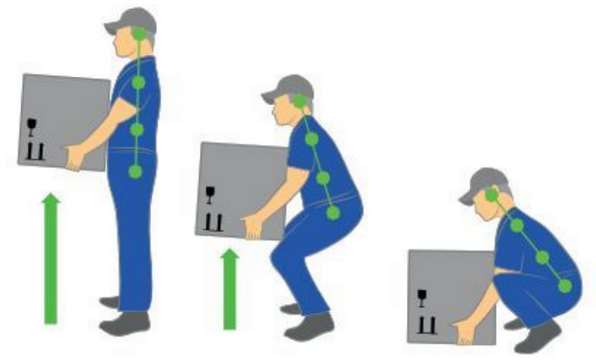
\includegraphics[scale=0.4]{../figs/G10-020-1}
\end{center}
\subsubsection{Biểu thức thế năng trọng trường}

Thế năng phụ thuộc vào vị trí của vật đối với vị trí được chọn làm mốc thế năng. 

Nếu chọn mốc thế năng trên mặt đất, khi một vật có khối lượng $m$ đặt ở độ cao $z$ so với mặt đất (trong trọng trường của Trái Đất) thì thế năng trọng trường của vật được xác định bằng:
\begin{equation*}
	W_\text{t}=mgz;
\end{equation*}
trong đó:
\begin{itemize}
	\item $W_\text{t}$ là thế năng trọng trường (có đơn vị là J);
	\item $m$ là khối lượng (có đơn vị là kg);
	\item $z$ là độ cao của vật so với mặt đất (có đơn vị là m).
\end{itemize}
Thế năng của vật trên mặt đất (vị trí mốc thế năng) bằng 0 ($z=0$). 

\subsubsection{Đặc điểm của thế năng trọng trường}

\begin{itemize}
	\item Thế năng là một đại lượng vô hướng có giá trị dương hoặc âm hoặc bằng không;
	\item Thế năng có tính tương đối, nghĩa là thế năng phụ thuộc vào vị trí ta chọn làm gốc thế năng;
	\item Trong bài toán chuyển động của vật, ta thường chọn gốc thế năng là tại mặt đất hoặc vị trí thấp nhất trên quỹ đạo của vật.
\end{itemize}
\subsubsection{Liên hệ giữa độ công trọng lực và độ giảm thế năng}

Khi một vật chuyển động trong trọng trường từ vị trí M đến vị trí N thì công của trọng lực của vật có giá trị bằng hiệu thế năng trọng trường tại M và N
\begin{equation*}
	A_\text{MN}=W_{\text{tM}}-W_{\text{tN}};
\end{equation*}
trong đó:
\begin{itemize}
	\item $A_\text{MN}$ là công của trọng lực;
	\item $W_{\text{tM}}$ và $W_{\text{tN}}$ lần lượt là thế năng tại M và thế năng tại N.
\end{itemize}

\textit{Hệ quả:} Trong quá trình chuyển động của một vật trong trọng trường:

\begin{itemize}
	\item Khi vật giảm độ cao, thế năng của vật giảm thì trọng lực sinh công dương.
	\item Khi vật tăng độ cao, thế năng của vật tăng thì trọng lực sinh công âm.
\end{itemize}
\section{Mục tiêu bài học - Ví dụ minh họa}
\begin{dang}{Tính động năng của một vật}
	\viduii{2}{Một vật có khối lượng $\SI{0.5}{kg}$ chuyển động với vận tốc $\SI{10}{m/s}$. Động năng của vật bằng
		\begin{mcq}(4)
			\item $\SI{250}{J}$.
			\item $\SI{50}{J}$.
			\item $\SI{5}{J}$.
			\item $\SI{25}{J}$.
		\end{mcq}
	}
	{\hide{		Động năng của vật: $W_\text{đ} = \dfrac{1}{2}mv^2 =\dfrac{1}{2}\cdot\SI{0.5}{\kilogram}\cdot(\SI{10}{\meter/\second})^2= \SI{25}{J}$.
		
		\textbf{Đáp án: D.}}
	}
	\viduii{2}{Một vận động viên có khối lượng $\SI{80}{kg}$ chạy đều hết quãng đường $\SI{180}{m}$ trong thời gian 40 giây. Động năng của vận động viên đó là
		\begin{mcq}(4)
			\item $\SI{810}{J}$. 
			\item $\SI{360}{J}$.
			\item $\SI{875}{J}$.
			\item $\SI{180}{J}$.
		\end{mcq}
	}
	{\hide{
		Vận tốc của vận động viên:
		$$v=\dfrac{s}{t} =\dfrac{\SI{180}{\meter}}{\SI{40}{\second}}= \SI{4.5}{\meter/\second}.$$
		
		Động năng của vận động viên:
		$$W_\text{đ} = \dfrac{1}{2} mv^2 =\dfrac{1}{2}\cdot\SI{80}{\kilogram}\cdot(\SI{4.5}{\meter/\second})^2= \SI{810}{J}.$$
		
		\textbf{Đáp án: A.}
		
	}
	}
\end{dang}

\begin{dang}{Tính độ biến thiên động năng}
	\viduii{2}{Một ô tô khối lượng $m$ bằng 1 tấn đang chuyển động với vận tốc $v=\SI{20}{m/s}$. Tính độ biến thiên động năng của ô tô khi nó bị hãm tới khi vận tốc còn $\SI{10}{m/s}$.
	}
	{\hide{
		Độ biến thiên động năng:
		\begin{align*}
			\Delta W_\text{đ} &= \dfrac{1}{2}mv^2-\dfrac{1}{2}mv_0^2\\
			&=\dfrac{1}{2}\cdot\SI{1000}{\kilogram}\cdot(\SI{10}{\meter/\second})^2-\dfrac{1}{2}\cdot\SI{1000}{\kilogram}\cdot(\SI{20}{\meter/\second})^2\\
			&= \SI{-150000}{J}=\SI{-150}{\kilo\joule}.
		\end{align*}
		
	}
	}
	\viduii{2}{Một lực $F$ không đổi làm một vật bắt đầu chuyển động và đạt được vận tốc $v$ sau khi đi được quãng đường $s$. Nếu tăng lực tác dụng lên 3 lần thì vận tốc của nó sẽ gấp bao nhiêu lần so với $v$? Cho biết quãng đường trong hai trường hợp đều là $s$.
	}
	{\hide{
		Áp dụng định lý động năng:
		\begin{equation*}
			A=Fs= \dfrac{1}{2}mv^2-\dfrac{1}{2}mv_0^2 = \dfrac{1}{2}mv^2 \Rightarrow v =\sqrt{\dfrac{2  F  s}{m}}.
		\end{equation*}
		Biểu thức trên cho thấy vận tốc tỉ lệ với căn bậc hai của lực, do đó khi lực tăng lên 3 lần thì vận tốc tăng $\sqrt{3}$ lần.
		
	}
	}
\end{dang}

\begin{dang}{Áp dụng định lí động năng}
	\viduii{3}{Một xe khối lượng 1 tấn khởi hành không vận tốc đầu, chuyển động nhanh dần đều trên đường nằm ngang. Sau khi đi được quãng đường $\SI{100}{m}$ thì đạt vận tốc $\SI{72}{km/h}$. Biết lực ma sát bằng $5\%$ trọng lượng của xe. Dùng định lý động năng, tính công của lực kéo của động cơ xe.
	}
	{\hide{
		Lực ma sát có độ lớn:
		$$F_\text{ms} = 5\%\cdot mg = 5\%\cdot\SI{1000}{\kilogram}\cdot\SI{10}{\meter/\second^2}=\SI{500}{N}.$$
		
		Áp dụng định lý động năng, độ biến thiên động năng bằng tổng công của các lực:
		\begin{align*}
			A_F + A_\text{ms} &= \dfrac{1}{2}mv^2 - 0\\ \Rightarrow\quad A_F &= \dfrac{1}{2} mv^2 - (-F_\text{ms}s) \\
			&=\dfrac{1}{2}\cdot\SI{1000}{\kilogram}\cdot(\SI{20}{\meter/\second})^2-(-\SI{500}{\newton}\cdot\SI{100}{\meter})\\
			&= \SI{250000}{J}\\
			&=\SI{250}{\kilo\joule}.		
		\end{align*}
		
	}
	}
	\viduii{3}{
		Một ô tô có khối lượng 2 tấn đang chạy với vận tốc $\SI{54}{km/h}$ trên đường nằm ngang thì lái xe thấy có chướng ngại vật cách ô tô $\SI{100}{m}$ thì tắt máy, đạp thắng. Biết hệ số ma sát giữa bánh xe và mặt đường là $\mu = 0,1$. Xe ô tô có đâm vào chướng ngại vật không? Cho $g=\SI{10}{m/s^2}$.
	}
	{\hide{
		Đơn vị vận tốc được đổi sang hệ SI: $$\SI{54}{\kilo\meter/\hour}=\dfrac{\SI{54e3}{\meter}}{\SI{3600}{\second}}=\SI{15}{\meter/\second}.$$
		
		Lực ma sát có độ lớn:
		\begin{align*}
			F_\text{ms}=\mu mg=\SI{0.1}{}\cdot\SI{2000}{\kilogram}\cdot\SI{10}{\meter/\second^2}=\SI{2000}{\newton}.
		\end{align*}
		Quãng đường xe chạy được cho đến khi dừng hẳn theo lý thuyết định lý động năng là:
		$$-F_\text{ms}s = 0 - \dfrac{1}{2}mv^2 \quad\Rightarrow\quad s = \dfrac{mv^2}{2F_\text{ms}}=\dfrac{\SI{2000}{\kilogram}\cdot(\SI{15}{\meter/\second})^2}{2\cdot\SI{2000}{\newton}}=\SI{112.5}{m}.$$
		
		Thực tế ô tô chỉ cách chướng ngại vật $\SI{100}{m}$ nên ô tô sẽ đâm vào chướng ngại vật trước khi kịp dừng lại.
	}
		}
	\viduii{4}{
		Một ô tô có khối lượng 2 tấn đang chuyển động trên đường thẳng nằm ngang AB dài $\SI{100}{\meter}$, khi qua A vận tốc ô tô là $\SI{10}{\meter/\second}$ và đến B vận tốc của ô tô là $\SI{20}{\meter/\second}$. Biết độ lớn của lực kéo là $\SI{4000}{\newton}$.
		\begin{enumerate}[label=\alph*)]
			\item Tìm hệ số ma sát $\mu_1$ trên đoạn đường AB.
			\item Đến B thì động cơ tắt máy và lên dốc BC dài $\SI{40}{\meter}$ nghiêng $30^\circ$ so với mặt phẳng ngang. Hệ số ma sát trên mặt dốc là $\mu_2=\dfrac{1}{5\sqrt{3}}$. Hỏi xe có lên đến đỉnh dốc C không?
			\item Nếu đến B với vận tốc trên, muốn xe lên dốc và dừng lại tại C thì phải tác dụng liên tục lên xe một lực có độ lớn bao nhiêu?
		\end{enumerate}
	}
	{\hide{
		\begin{enumerate}[label=\alph*)]
			\item 
			
			Áp dụng định lý động năng:
			$$-\mu_1 mg s_1 + Fs_1 = \dfrac{1}{2}mv_\text{B}^2 - \dfrac{1}{2}mv_\text{A}^2 \Rightarrow \mu_1 = \SI{0.05}{}.$$
			\item 			
			Áp dụng định lý động năng từ B đến khi xe dừng lại:
			$$A_\text{ms2}+A_{P2} = 0 - \dfrac{1}{2}mv_\text{B}^2 \Rightarrow -\mu_2 mg \cos \alpha s_2 - mgs_2 \sin \alpha = 0 - \dfrac{1}{2}mv_\text{B}^2 \Rightarrow s_2 = \SI{33.33}{m}.$$
			
			Vậy quãng đường tối đa xe lên được là $\SI{33.33}{m}$, mà dốc dài $\SI{40}{m}$ nên xe không lên được đến đỉnh dốc.
			\item 			
			Để xe lên được đến C thì $s_3=\SI{40}{m}$, khi đó:
			$$A_\text{ms3}+A_{P3}+A_F = 0 - \dfrac{1}{2}mv_\text{B}^2$$ $$\Rightarrow -\mu_2 mg \cos \alpha s_3 - mgs_3 \sin \alpha +Fs_3= 0 - \dfrac{1}{2}mv_\text{B}^2 \Rightarrow F = \SI{1}{N}.$$
		\end{enumerate}
	}}
\end{dang}
\begin{dang}{Xác định thế năng của vật trong trọng trường}
	\viduii{2}{Một vật có khối lượng $\SI{2}{kg}$ được thả rơi từ độ cao $\SI{4.5}{m}$ xuống mặt đất, tại nơi có gia tốc trọng trường là $\SI{10}{m/s^2}$. Xác định thế năng của vật trong trường hợp chọn gốc thế năng tại mặt đất.
	}
	{\hide{
		Chọn gốc thế năng tại mặt đất. Thế năng của vật:
		$$W_\text t = mgz = \SI{2}{\kilogram}\cdot\SI{10}{\meter/\second^2}\cdot\SI{4.5}{\meter}=\SI{90}{J}.$$
	}
	}
	\viduii{2}{Một vật có khối lượng $\SI{10}{\kilogram}$, lấy $\SI{10}{\meter/\second^2}$. Tính thế năng của vật tại A cách mặt đất $\SI{3}{m}$ về phía trên và tại đáy giếng B cách mặt đất $\SI{5}{m}$ với gốc thế năng tại mặt đất.
	}
	{\hide{
		Thế năng của vật tại A cách mặt đất $\SI{3}{m}$ ($z_\text{A}=\SI{3}{m}$) là:
		\begin{equation*}
			W_{\text{tA}}=mgz_\text{A}=\SI{10}{\kilogram}\cdot\SI{10}{\meter/\second^2}\cdot\SI{3}{m}=\SI{300}{\joule}.
		\end{equation*}
		
		Thế năng của vật tại đáy giếng B cách mặt đất $\SI{5}{m}$ ($z_\text{B}=-\SI{5}{m}$) là:
		\begin{equation*}
			W_{\text{tB}}=mgz_\text{B}=\SI{10}{\kilogram}\cdot\SI{10}{\meter/\second^2}\cdot(-\SI{5}{m})=\SI{-500}{\joule}.
		\end{equation*}
		
	}
	}
	\viduii{3}{Một học sinh thả một vật rơi tự do có khối lượng $\SI{500}{\gram}$ từ độ cao $\SI{45}{\meter}$ so với mặt đất, bỏ qua ma sát với không khí. Tính thế năng của vật tại giây thứ hai so với mặt đất. Cho $g= \SI{10}{\meter/\second^2}$.
	}
	{\hide{
		Độ cao của vật tại giây thứ hai so với mặt đất:
		$$h_2 = h - \dfrac{1}{2}gt^2 = \SI{25}{m}.$$
		
		Chọn gốc thế năng tại mặt đất. Thế năng của vật tại thời điểm đó:
		$$W_\text t = mgh_2 = \SI{0.5}{\kilogram}\cdot\SI{10}{\meter/\second^2}\cdot\SI{25}{\meter}=\SI{125}{J}.$$
	}
	}
\end{dang}

\begin{dang}{Vận dụng liên hệ giữa công của trọng lực và độ giảm thế năng }
	
	\viduii{2}{
		Một vật có khối lượng $\SI{100}{\gram}$ đang ở độ cao $\SI{6}{\meter}$ so với mặt đất. Tìm công của trọng lực tác dụng lên vật khi vật rơi đến độ cao $\SI{2}{\meter}$.
	}
	{\hide{
		Chọn gốc thế năng tại mặt đất.
		
		Công của trọng lực tác dụng lên vật khi vật rơi từ độ cao $\SI{6}{\meter}$ đến độ cao $\SI{2}{\meter}$ là:
		\begin{equation*}
			A=W_{\text{t}1}-W_{\text{t}2}=mgz_1-mgz_2=mg(z_1-z_2)=\SI{0,1}{\kilogram}\cdot\SI{10}{\meter/\second^2}\cdot(\SI{6}{\meter}-\SI{2}{\meter})=\SI{4}{\joule}.
		\end{equation*}
	}
		}
	\viduii{3}{
		Một người thực hiện công đạp xe đạp lên đoạn đường dài $\SI{40}{\meter}$ trên một dốc nghiêng $20^\circ$ so với phương ngang. Bỏ qua mọi ma sát. Nếu thực hiện một công cũng như vậy mà lên dốc nghiêng $30^\circ$ so với phương ngang thì người đó sẽ đi được đoạn đường bao nhiêu?
	}
	{
		\hide{
		Chọn gốc thế năng tại mặt đất.
		
		Nếu bỏ qua mọi ma sát, thì công tối thiểu người này cần thực hiện lên dốc bằng công của trọng lực
		\begin{align*}
			A&=mgh=mgl_1\sin\alpha_1=mgl_2\sin\alpha_2\\
			\Rightarrow\quad l_2&=\dfrac{l_1\sin\alpha_1}{\sin\alpha_2}=\dfrac{\SI{40}{\meter}\cdot\sin 20^\circ}{\sin 30^\circ}\approx\SI{27,36}{\meter}.
		\end{align*}
	}}
\end{dang}